\chapter{Discussion\label{ch:disc}}

As expected, gender is a significant determinant in the general model for entrepreneurship, as seen in the first column of Table B.1. The most important other factors for this model are education, income, immigrant status, skill versatility, minority group, marriage status and industry-specific effects. While some determinants abide by our formulated hypotheses in the probit coefficients they produce (income, age, skill versatility), others provide significantly different results than those anticipated (marital status, immigrant status). Results for all significant covariates across the three samples can be visualized in Figure B.1 [Regression Results]. In comparing the general model with the gendered-differentiated ones, we note the standard empirical approach to investigating the determinants of business entry ignores important asymmetries between men and women's responsiveness to policy, macroeconomic conditions or individual characteristics that might lead to business formation. 

\section{Availability of Capital}
Our findings highlight that women are positively, but to a lesser degree than men motivated by capital upon starting a business. This might speak to a certain degree of risk aversion observed in women more than in men\footnote{\cite{adams2012beyond} observe that women do not take as many risks at the workplace as men do, in an attempt to avoid being perceived poorly by colleagues. This behavioral pattern disappears when authors look at female CFO's, indicating that arriving at this leadership position allows women to suppress perception concerns. In turn, female CFO's are observed to be just as, and often times even more risk-taking than their male counterparts.}, which can echo in investment decisions and allocation of current income. If women are less risk-taking in the aggregate, then they might not perceive monetary surplus as a chance to start their own company, and think instead in longer-term frameworks. Our finding then suggests that from a policy standpoint, infusions of liquidity might not have immediate effects in spurring female entrepreneurship. 

\section{Education and Skills}
We predicted higher education would lessen incentives for immigrant men and women to start companies, as an indicator of the demand for their wage-labor at a given time. The effect on business formation was indeed negative, but smaller in magnitude for immigrant women than for men. One explanation is that women in immigrant groups might still encounter less demand for their wage labor than their male counterparts, despite having similar levels of educational attainment\footnote{\cite{ReynoldsWhite1997}}. If their work is not rewarded to a similar extent for highly educated immigrant women to prefer wage employment to opening a business, this adds to the observation that the U.S. labor market doesn't offer equal opportunities across genders.

Regarding the mixed effects of education, we hypothesized that in times of economic upturn, highly educated agents will be less likely to start a business for similar demand-side reasons as those invoked above. While this effect was found to be negative in the aggregate, education was less likely to deter self-employment in periods of economic upturn in the case of women. This finding could suggest labor market discrimination, but might also substantiate the risk-aversion theory in making women less likely to respond immediately to favorable changes in economic conditions.

Our results provide direct empirical evidence that skill versatility matters to a greater extent than the level of education, a claim speculated in theoretical frameworks for entrepreneurship\footnote{\cite{Lazear2005}}, but not fully analyzed in empirical research. This robust finding holds across genders, with the ability to change industries having positive effects on the probability of self-employment. 

\section{Marriage}

We found that marital status does not produce the positive effects suggested across self-employment literature, with most positive coefficients observed for those who have never been married. The theories of supportive spouses\footnote{ Referring to the idea that married couples are more likely to open businesses due to more access to capital, as well as the option to work for the new company at below-market rates.}, tax benefits and below-market price labor could still hold, but the incentives for single people to start businesses are equally, if not more prominent. While the view of the risk taking, lone entrepreneur might find some backing in these results, a more realistic interpretation relies on the power of professional networks, friend groups and support that goes beyond one's life partner in facilitating business ventures. 

\section{Minority Group}

The coefficients across minority groups indirectly reveal the significant extent to which African-Americans, Hispanics or American-Indians are held back in the U.S. labor market when it comes to starting a business. In that sense, the negative estimates confirmed our expectations, with the only group experiencing positive effects on entrepreneurship entry being Asian Americans. Across the minority groups for which business formation is less likely, women were observed to experience a slightly smaller negative effect. An explanation might consist of a smaller degree of stigma associated with women in these groups when compared to their male counterparts\footnote{\cite{AlbaRumbautMarotz2005}}, which could translate to less expected barriers in accessing funding and resources. 

\section{Lifestyle Choices}
Lifestyle choices motivating entrepreneurship also differ for men and women, with men being more likely to switch to self-employment if it implies less hours worked, while women experience the reverse. This adds nuance to assumptions in existing literature, which denote women might choose self-employment for the flexibility benefits and ability to work less\footnote{\cite{bertrand2013gender}}. Marital status is not able to substantiate this claim, suggesting there is more to the story of some married women opening a business to have more time for household work. To that end, women might regard self-employment as a leadership opportunity and as a response to barriers in advancement encountered in wage-employment\footnote{\cite{olivetti2016dp11034}}. Therefore, they invest time and effort into running their own company, and demonstrate a high time commitment throughout. Men might not develop similar incentives, viewing self-employment as a transitioning state, or as an activity providing a more flexible lifestyle. It is important to note our data targets individuals in metropolitan and non-metropolitan areas across the U.S., which can differ in terms of gender attitudes. 


\section{Industry Effects}

Industries remain similarly segregated as in the case of wage employment, with women not being able to penetrate traditionally male-dominated fields by the act of opening a business. Software engineering, data processing or internet services attract men to a significantly greater degree than the sample average, while industries like apparel, real estate or accounting tend to motivate female presence [illustrated in Figure 6.1 below]. Although women are just as likely to change industry upon joining self-employment as men, there are still differences in the fields they choose. 

This finding could be partially explained by differences in field of study across genders, with women underrepresented in science and technology subjects at similar level of educational attainment\footnote{\cite{olivetti2016dp11034}}. It could also mean certain barriers in wage employment\footnote{Some examples include less representation, barriers to entry, barriers to advancement, wage discrimination.} get transferred to self-employment, and that opening one's business describes an unrealistic mechanism for surpassing existing deterrents. 

\begin{figure}[hbtp]
	  \centering{%
		  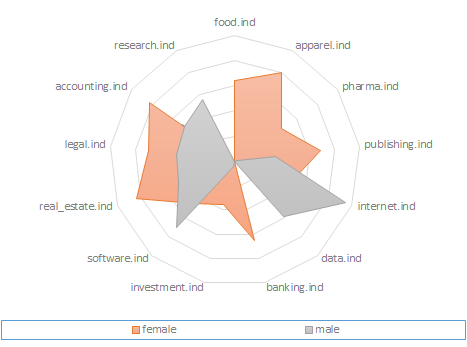
\includegraphics[width=0.7\linewidth]{ch-discussion/industry_fm.png}%
    	}%
    \caption{Magnitude of Positive Industry Coefficients by Gender} 
\end{figure}

\section{Economic Conditions}

In terms of environment variables, men were found to be more responsive to macroeconomic conditions, while women tend to be motivated to a greater degree by tax credits. The first finding might speak to how genders perceive changes in local economies\footnote{Research on this topic is not comprehensive, but some insights are provided by \cite{LeachHayhoeTurner1999}, who look at how female and male college students perceive their own economic well-being differently, with differential effects across factors. Difference in behaviors that originate in perceived economic well-being have also been studied, some examples being credit card use \cite{armstrong1993credit} or spending habits \cite{LeachHayhoeTurner1999}.}, but also the degree to which they are allowed to flexibly adapt to them. If women's degree of labor mobility is more limited, awareness of periods of economic boom might not automatically translate to better opportunities in wage employment and less motivation to start a business. 

On the tax side, women's responsiveness to these types of policies might attest to their efficiency in targeting prospective female business owners, but also a different outlook for this particular group. Specifically, responsiveness to tax credits might point to a long-term focus in planning and more responsibility as household providers/caretakers in the case of women. In this light, men's responsiveness to current economic conditions would indicate a more short-term approach, with planning to echo current business indicators. 

\section{Political Climate}
Our findings regarding political climate highlight that women tend to be motivated to start a business if they have a democratic governor, and experience negative effects from republican local governance. One assumption underlying this result might have to do with policies attributed to both parties, and their differential appeal to female voters. It might be that democratic measures encourage a better business climate for women, with policies targeting work-life balance that have no effect on men's considerations. 

Similarly, although the Republican party is associated with tax breaks and a friendlier regulatory regime, small businesses haven't historically been the center of republican measures, with bigger companies thought to stand at the core of republican policies\footnote{\cite{Brown2010}}. Since new businesses often start small, this can influence women's perception of the business climate in their given state if associated with Republican governance. If an agent's sense of worth and perception of risk are \textit{gendered qualities}\footnote{Here, we refer to different perceptions of risk and self-worth explored by psychological work.}\hspace{.15em}\footnote{\cite{adams2012beyond}}, this would further explain why men would not be affected by this policy focus, and why it makes a significant negative difference for women.

Nonetheless, we find no significance to partisanship \textit{changes} at the local level, which could point to an alternative interpretation of the results. If the leadership climate is merely a reflection of the voter base, then states that are historically republican-governed might correspond to different attitudes about policy, business ownership and gender roles. The partisanship of the governor can thus be an instrument that measures gender attitudes at the local level, attitudes that affect the number of women that might pursue entrepreneurship at a given time. This is in line with the lack of statistical significance for partisanship change at the local level, pointing that transitions in governance might not matter as much as the general ideology of a region.

\section{Robustness Check}

\subsection{External Validity}

Our models were able to capture a significant proportion of the variability in self-employment entry, with Pseudo $R^2$ coefficients surpassing 0.5. There are however, areas that could benefit from further exploration, a more comprehensive set of variables being expected to add to the current research in insightful ways. 

In terms of education and its effect on self-employment rates, it is known that in most OECD countries men and women reach similar attainment levels\footnote{\cite{charles2002equal}}. However, there is a persistent gender gap in \textit{educational choices} across genders, with women being a majority in fields like health and education, and underrepresented in more technical programs, like hard sciences and engineering\footnote{\cite{charles2002equal}}. Given that our data doesn't capture field of study, but only level of educational attainment and industry of choice, one can suspect that similar education level might not bring the same effects across individuals, especially since technical fields are more often associated with both entrepreneurship of innovation, as well as persistent gender gaps. 

Entrepreneurship is often associated with \textit{``greater flexibility in terms of an agent's discretion over the length, location and scheduling of their work time''}\footnote{\cite{Quinn1980}}. It is thus expected for people with poor health or disabilities to have a higher probability of self-employment, as a way to avoid workplace discrimination\footnote{\cite{Quinn1980}}. The relation between self-employment and ill-health or disability could be an important control for self-employment decisions, one to be explored with more generous data. 

Research\footnote{ Works by \cite{BurkeFitzroyNolan2002}; \cite{GeorgellisWall2005} or \cite{CowlingTaylor2001} do not treat the number of children an agent has as the covariate of interest, but use it as a control.} also finds that children act as a greater impediment on a female's entrepreneurial career than that of a male, a factor our model does not control for due to data limitations. In the future, the role of children on parents' decisions to become entrepreneurs, as well as quit self-employment could be studied to capture whether changes of societal perceptions on parenthood have occurred, or whether traditional parenting patterns are still in place.  













